\documentclass{article}
\usepackage{amsmath}
\usepackage{algorithm}
\usepackage{algpseudocode}
\usepackage{pdflscape}
\usepackage{graphicx}
\usepackage{blindtext}
\usepackage{booktabs}
\usepackage{breqn}
\usepackage{algcompatible}
\usepackage{float}
\usepackage{dutchcal}
\usepackage{amsfonts}

\def\bSig\mathbf{\Sigma}
\newcommand{\VS}{V\&S}
\newcommand{\tr}{\mbox{tr}}

\begin{document}

\section*{Supplementary Materials}

\subsection{Glossary of Notation}

\begin{itemize}

    \item $\mathbf{Y}$: A $n \times J$ matrix containing all multivariate skew-normal  outcomes such that $y_{ij}$ is the $j^{th}$ outcome observed for subject $i$, where $i = 1,...,n$ and $j = 1,...J$.
    
    \item $\mathbf{X}$: A $n \times P$ matrix containing all multivariate skew-normal regression covariates such that $x_{ip}$ is the $p^{th}$ covariate value for subject $i$, where $i = 1,...,n$ and $p = 1,...P$.
    
    \item $\mathbf{B}$: A $P \times J$ matrix containing all multivariate skew-normal regression coefficients such that $\mathbf{B} = \left [ \boldsymbol\beta_1,...,\boldsymbol\beta_J \right ]$, where $\beta_{pj}$ is interpreted as the effect of covariate $p$ on outcome $j$ for $p = 1,...,P$ and $j = 1,...,J$.
    
    \item $\mathbf{E}$: A $n \times J$ matrix of error terms in the multivariate skew-normal regression model component. $\mathbf{E}$ is made up of row vectors $\boldsymbol\epsilon_i = (\epsilon_{i1},...,\epsilon_{iJ})$, where $ \boldsymbol\epsilon_i \stackrel{iid}{\sim} N_J(0, \boldsymbol\Sigma)$ for $i = 1,...,n$.
    
    \item $\boldsymbol\Sigma$: A $J \times J$ covariance matrix that defines the correlation between the $p$ multivariate normal outcomes. 
    
    \item $\boldsymbol\Omega$: A $J \times J$ covariance scale matrix that defines the correlation between the $p$ multivariate skew-normal outcomes. 
    
    \item $\boldsymbol\psi$: A $J \times 1$ vector containing the skewness parameter for each outcome.
    
    \item $\boldsymbol\alpha$: A $J \times 1$ vector containing the skewness parameter for each outcome.
    
    \item $\mathbf{t}$: An $n \times 1$ vector of truncated normal random effects used in the stochastic representation of the multivariate skew-normal distribution. For $i = 1,...,n$, $t_i \stackrel{iid}{\sim}T_{[0,\infty)}(0,1)$
    
    \item $\mathbf{X}^*$: A $n \times (P + 1)$ matrix constructed by column binding $\mathbf{t}$ to $\mathbf{X}$
    
    \item $\mathbf{B}^*$: A $(P+1) \times J$ matrix constructed by row binding $\boldsymbol\psi^T$ to $\mathbf{B}$.

\end{itemize}

\newpage
\subsection{Derivations of Full Conditional Distributions}

\subsubsection{Multivariate Skew-Normal Regression}

Without loss of generality, we derive the full conditional distributions for the multivariate skew-normal regression model component under the assumption that all observations belong to a single cluster. To make the extension to the case where more than one cluster is specified, simply apply these distributional forms to cluster specific parameters and data. Finally, we assume for the moment that we have complete data for all outcomes for each subject. We extend consider the case of missing data in section (INSERT SECTION).

The multivariate skew-normal regression model can be written as follows in matrix form. 
$$\mathbf{Y} = \mathbf{X}\mathbf{B} + \mathbf{t} \boldsymbol\psi^T + \mathbf{E} = \mathbf{X}^* \mathbf{B}^* + \mathbf{E}$$
The matrix $\mathbf{Y}$ is of dimension $n \times J$. For convenience, we define $\mathbf{X}^*$ as a $n \times (P + 1)$ matrix constructed by column binding $\mathbf{t}$ to $\mathbf{X}$, and $\mathbf{B}^*$ as a $(P+1) \times J$ matrix constructed by row binding $\boldsymbol\psi^T$ to $\mathbf{B}$. We assume that $t_i \stackrel{iid}{\sim}T_{[0,\infty})(0,1)$ and that $\mathbf{E}$ is made of row vectors $\boldsymbol\epsilon_i = (\epsilon_{i1},...,\epsilon_{iJ})$ for $i = 1,...,n$, where $ \boldsymbol\epsilon_i \stackrel{iid}{\sim} N_J(0, \boldsymbol\Sigma)$.

The conditional likelihood for this model is given below. 
$$p(\mathbf{Y}|\mathbf{X}^*,\mathbf{B}^*,\boldsymbol\Sigma) \propto |\boldsymbol\Sigma|^{-n/2}\exp \left \{ -\frac{1}{2} \tr(\mathbf{Y} - \mathbf{X}^* \mathbf{B}^*)^T(\mathbf{Y} - \mathbf{X}^* \mathbf{B}^*)\boldsymbol\Sigma^{-1} \right \}$$

We choose conjugate priors for $\mathbf{B}^*$ and $\boldsymbol\Sigma$ as follows. 
$$\boldsymbol\Sigma \sim \text{inverse-Wishart}(\mathbf{V}_0,\nu_0)$$
$$\mathbf{B}^*|\boldsymbol\Sigma \sim MatNorm_{(m+1), p}(\mathbf{B}_0^*,\mathbf{L}_0^{-1},\boldsymbol\Sigma)$$

We now derive the joint posterior distribution of the parameters $\mathbf{B}^*$ and $\boldsymbol\Sigma$.
\begin{align*} 
p(\mathbf{B}^*,\boldsymbol\Sigma|\mathbf{X}^*,\mathbf{Y}) & \propto  p(\mathbf{Y}|\mathbf{X}^*,\mathbf{B}^*,\boldsymbol\Sigma)p(\mathbf{B}^*|\boldsymbol\Sigma)p(\boldsymbol\Sigma)\\
&  \propto |\boldsymbol\Sigma|^{-n/2}\exp \left \{ -\frac{1}{2} \tr \left [(\mathbf{Y} - \mathbf{X^*}\mathbf{B}^*)^T(\mathbf{Y} - \mathbf{X^*}\mathbf{B}^*)\boldsymbol\Sigma^{-1} \right ]\right \} \\
& \times |\boldsymbol\Sigma|^{-(P+1)/2} \exp \left \{ -\frac{1}{2} \tr \left [(\mathbf{B}^* - \mathbf{B}^*_0)^T \mathbf{L}_0(\mathbf{B}^* - \mathbf{B}^*_0)\boldsymbol\Sigma^{-1} \right ]\right \} \\
& \times |\boldsymbol\Sigma|^{(\nu_0 + J + 1)/2} \exp \left \{ -\frac{1}{2} \tr (\mathbf{V}_0 \boldsymbol\Sigma^{-1}) \right \}
\end{align*}



\subsubsection{Multinomial Logit Regression}

\subsubsection{Multivariate Normal Conditional Imputation}

The multivariate normal conditional imputation derivations are given for a single cluster without loss of generality. In practice, the data and parameters in this section would be replaced by cluster specific estimates in the case of clustering. 

For a given observation vector $\mathbf{y} \sim N_J(\boldsymbol\mu, \boldsymbol\Sigma)$, we allow for missingness in at most $J - 1$ of the multivariate outcomes through the use of a conditional imputation step embedded within our Gibbs sampler. Suppose $\mathbf{y}$ contains $q$ missing observations and can be partitioned into two vectors $\mathbf{y_{1}}$ and $\mathbf{y_{2}}$ such that $\mathbf{y_{1}}$ is a $q \times 1$ vector of missing observations and $\mathbf{y_{2}}$ is a $(J-q) \times 1$ vector of complete observations. Similarly, partition $\boldsymbol\mu$ and $\boldsymbol\Sigma$ as follows.
$$\boldsymbol\mu = \begin{bmatrix} \boldsymbol\mu_1 \\ \boldsymbol\mu_2 \end{bmatrix} \ \ \ \ \ \boldsymbol\Sigma = \begin{bmatrix} \boldsymbol\Sigma_{11} & \boldsymbol\Sigma_{12} \\ \boldsymbol\Sigma_{21} & \boldsymbol\Sigma_{22} \end{bmatrix}$$

We will use these quantities to derive the conditional distribution $f(\mathbf{y_1}|\mathbf{y_2},\boldsymbol\mu,\boldsymbol\Sigma)$. 
\begin{align*} 
f(\mathbf{y_1}|\mathbf{y_2},\boldsymbol\mu,\boldsymbol\Sigma) & \propto  f(\mathbf{y_1},\mathbf{y_2}|\boldsymbol\mu,\boldsymbol\Sigma) \\
& \propto \exp \left \{ -\frac{1}{2}(\mathbf{y} - \boldsymbol\mu)^T \boldsymbol\Sigma^{-1} (\mathbf{y} - \boldsymbol\mu) \right \} \\
& = \exp \left \{ -\frac{1}{2}\begin{bmatrix} \mathbf{y}_1 - \boldsymbol\mu_1 \\  \mathbf{y}_2 - \boldsymbol\mu_2 \end{bmatrix}^T \boldsymbol\Sigma^{-1} \begin{bmatrix} \mathbf{y}_1 - \boldsymbol\mu_1 \\  \mathbf{y}_2 - \boldsymbol\mu_2 \end{bmatrix} \right \} \\
& =  \exp \left \{ -\frac{1}{2}\begin{bmatrix} \mathbf{y}_1 - \boldsymbol\mu_1 \\  \mathbf{y}_2 - \boldsymbol\mu_2 \end{bmatrix}^T \begin{bmatrix} \boldsymbol\Sigma_{11} & \boldsymbol\Sigma_{12} \\ \boldsymbol\Sigma_{21} & \boldsymbol\Sigma_{22} \end{bmatrix}^{-1} \begin{bmatrix} \mathbf{y}_1 - \boldsymbol\mu_1 \\  \mathbf{y}_2 - \boldsymbol\mu_2 \end{bmatrix} \right \} \\
& = \exp \left \{ -\frac{1}{2}\begin{bmatrix} \mathbf{y}_1 - \boldsymbol\mu_1 \\  \mathbf{y}_2 - \boldsymbol\mu_2 \end{bmatrix}^T \begin{bmatrix} \boldsymbol\Sigma_{11}^* & \boldsymbol\Sigma_{12}^* \\ \boldsymbol\Sigma_{21}^* & \boldsymbol\Sigma_{22}^* \end{bmatrix} \begin{bmatrix} \mathbf{y}_1 - \boldsymbol\mu_1 \\  \mathbf{y}_2 - \boldsymbol\mu_2 \end{bmatrix} \right \} \\
& = \exp \left \{ -\frac{1}{2} \left[ (\mathbf{y}_1 - \boldsymbol\mu_{cond})^T \boldsymbol\Sigma_{cond}^{-1}(\mathbf{y}_1 - \boldsymbol\mu_{cond})\right]\right \} 
\end{align*}
$$\Rightarrow \mathbf{y_1}|\mathbf{y_2},\boldsymbol\mu,\boldsymbol\Sigma \sim N_q(\boldsymbol\mu_{cond},\boldsymbol\Sigma_{cond})$$
$$\boldsymbol\mu_{cond} = \boldsymbol\mu_1 + \boldsymbol\Sigma_{12}\boldsymbol\Sigma_{22}^{-1}(\mathbf{y}_2 - \boldsymbol\mu_2), \ \ \ \ \ \ \boldsymbol\Sigma_{cond} = \boldsymbol\Sigma_{11} - \boldsymbol\Sigma_{12}\boldsymbol\Sigma_{22}^{-1}\boldsymbol\Sigma_{21}$$

The block-wise inversion formula was used to invert $\boldsymbol\Sigma$ according to the following reparameterizations.
\begin{align*}
\boldsymbol\Sigma_{11}^* & = \boldsymbol\Sigma_{11}^{-1} + \boldsymbol\Sigma_{11}^{-1}\boldsymbol\Sigma_{12}(\boldsymbol\Sigma_{22} - \boldsymbol\Sigma_{21}\boldsymbol\Sigma_{11}^{-1}\boldsymbol\Sigma_{12})^{-1}\boldsymbol\Sigma_{21}\boldsymbol\Sigma_{11}^{-1}\\
\boldsymbol\Sigma_{12}^* & = -\boldsymbol\Sigma_{11} \boldsymbol\Sigma_{12}(\boldsymbol\Sigma_{22}-\boldsymbol\Sigma_{21}\boldsymbol\Sigma_{11}^{-1}\boldsymbol\Sigma_{12})^{-1}\\
\boldsymbol\Sigma_{21}^* & = -(\boldsymbol\Sigma_{22} - \boldsymbol\Sigma_{21}\boldsymbol\Sigma_{11}^{-1}\boldsymbol\Sigma_{12})^{-1}\boldsymbol\Sigma_{21}\boldsymbol\Sigma_{11}^{-1}\\
\boldsymbol\Sigma_{22}^* & = (\boldsymbol\Sigma_{22} - \boldsymbol\Sigma_{21}\boldsymbol\Sigma_{11}^{-1}\boldsymbol\Sigma_{12})^{-1}     
\end{align*}

\subsection{Tables}

\begin{algorithm}
\caption{Gibbs Sampler}
\label{alg:MCMC}
\begin{algorithmic}
\small
\linespread{0.5}
    \State $\mathbf{Define} \ n_{iter};\  n_{burn}; \ K; \ \boldsymbol\theta_{init}; \ \boldsymbol\theta_0$
    \State $n_{sim} := n_{iter} - n_{burn}$
    \State $\boldsymbol\theta := \boldsymbol\theta_{init}$
    \For {$\iota = 1,...,n_{sim}$}
        \State \textsc{I. Conditional Imputation}
          \For {$ i = 1,...,n$}
            \State $\mathbf{Draw} \ \mathbf{y}_i^{miss} \ \text{from} \ N_q(\boldsymbol\mu_i^{miss}, \boldsymbol\Sigma_i^{miss})$
            \State $\mathbf{y}_i := \mathbf{y}_i^{miss} \cup \mathbf{y}_i^{obs}$
         \EndFor
        \State \textsc{II. MSN Regression}
          \For {$ k = 1,...,K$}
            \State $n_k := \sum_{i = 1}^n {1}_{z_i = k}$
            \For {$i_k = 1,...,n_k$}
              \State $\mathbf{Draw}\  t_i \ \text{from} \ N_{[0,\infty)}(a_i,A)$
            \EndFor
            \State $\mathbf{X^*}_k := $ \texttt{cbind}$(\mathbf{X}_k,\mathbf{t}_k)$
            \State $\mathbf{Draw} \ \mathbf{B^*}_k \ \text{from} \ \text{MatNorm}(\mathbf{B}_k,\mathbf{L}_k^{-1},\boldsymbol\Sigma_k)$
            \State $\mathbf{Draw} \ \boldsymbol\Sigma_k \ \text{from} \ \text{InvWish}(\nu_k, \mathbf{V}_k)$
          \EndFor
        \State \textsc{III. Multinomial Logit}
          \For {$i = 1,...,n$}
            \For {$k = 1,...,K$}
              \State $\pi_{ik} := P(z_i = k|\mathbf{w}_i,\boldsymbol\delta_k)$
              \State $p_{ik} := P(\mathbf{y}_i|\boldsymbol\beta_k^{*T} \mathbf{x}^*_i,\boldsymbol\Sigma_k)$
            \EndFor
            \State $\mathbf{p}_{z_i} := \frac{\mathbf{p}_i \circ \boldsymbol\pi_i}{\mathbf{p}_i \cdot \boldsymbol\pi_i}$
            \State $\mathbf{Draw} \ z_i \ \text{from} \ \text{Categorical}(\mathbf{p}_{z_i})$
            \For {$k = 1,...,K-1$}
              \State $\mathbf{Draw} \ \boldsymbol\delta_k \ \text{from} \ N(\mathbf{M},\mathbf{S})$
            \EndFor
          \EndFor
        \State $\boldsymbol\theta := \{\mathbf{B^*}, \boldsymbol\Sigma, \mathbf{Z}, \boldsymbol\delta \}$
        \State $\mathbf{Store} \ \boldsymbol\theta$
	  \EndFor
\end{algorithmic}
\end{algorithm}


\begin{landscape}\begin{table}[t]

\caption{\label{tab:unnamed-chunk-5}Model results for simulated data with n = 1000, J = 4, p = 2, K = 3, r = 2. 1,000 iterations were run with a burn in of 100. The missingness mechanism was MAR and P(miss) = 0. Model results for the multivariate skew normal (MSN) and multivariate normal (MN) mixtures are presented. Intervals that do not contain the true parameter are denoted with (*).}
\centering
\fontsize{6}{8}\selectfont
\begin{tabular}{lllllllllll}
\toprule
\multicolumn{2}{c}{ } & \multicolumn{3}{c}{Class 1} & \multicolumn{3}{c}{Class 2} & \multicolumn{3}{c}{Class 3} \\
\cmidrule(l{3pt}r{3pt}){3-5} \cmidrule(l{3pt}r{3pt}){6-8} \cmidrule(l{3pt}r{3pt}){9-11}
Component & Param. & True & MSN Est. (95\% CrI) & MN Est. (95\% CrI)  & True & MSN Est. (95\% CrI) & MN Est. (95\% CrI) & True & MSN Est. (95\% CrI) & MN Est. (95\% CrI)\\
\midrule
\addlinespace[0.3em]
\multicolumn{11}{l}{\textbf{ }}\\
\hspace{1em}MSN & $\beta_{11}$ & -3.07 & -2.7 (-3.27, -2.34) & -3.44 (-3.76, -3.11)* & 0.42 & 0.9 (-0.06, 1.7) & 0.82 (0.45, 1.19)* & 2.46 & 2.23 (1.75, 2.56) & 1.3 (1.06, 1.54)*\\
\hspace{1em}Regression & $\beta_{21}$ & -2.04 & -1.99 (-2.17, -1.82) & -1.96 (-2.13, -1.8) & -0.31 & -0.26 (-0.44, -0.02) & -0.27 (-0.43, -0.08) & 3.26 & 3.27 (3.16, 3.38) & 3.28 (3.16, 3.4)\\
\hspace{1em} & $\beta_{31}$ & -3.03 & -3.14 (-3.55, -2.77) & -3.41 (-3.74, -3.08)* & 0.34 & 0.49 (-0.41, 1.35) & 0.62 (0.23, 0.94) & 2.93 & 2.77 (2.05, 3.09) & 1.82 (1.61, 2.07)*\\
\hspace{1em} & $\beta_{41}$ & -3.26 & -3.24 (-3.4, -3.07) & -3.25 (-3.42, -3.09) & -0.63 & -0.59 (-0.77, -0.38) & -0.6 (-0.76, -0.42) & 2.53 & 2.54 (2.43, 2.65) & 2.55 (2.45, 2.67)\\
\hspace{1em} & $\beta_{12}$ & -3.12 & -3.48 (-3.88, -2.82) & -3.44 (-3.71, -3.18)* & 0.09 & 0.51 (-0.32, 1.27) & 0.4 (0.04, 0.72) & 2.67 & 2.22 (1.29, 2.58) & 1.54 (1.31, 1.77)*\\
\hspace{1em} & $\beta_{22}$ & -2.61 & -2.62 (-2.77, -2.48) & -2.62 (-2.76, -2.5) & -0.37 & -0.35 (-0.52, -0.15) & -0.34 (-0.51, -0.18) & 2.1 & 2.07 (1.96, 2.18) & 2.08 (1.96, 2.18)\\
\hspace{1em} & $\beta_{32}$ & -2.84 & -2.8 (-3.4, -2.36) & -3.29 (-3.59, -2.97)* & -0.06 & 0.24 (-0.71, 1.12) & 0.26 (-0.1, 0.62)* & 1.89 & 1.57 (1.07, 1.87)* & 0.72 (0.51, 0.94)*\\
\hspace{1em} & $\beta_{42}$ & -2.8 & -2.62 (-2.79, -2.48)* & -2.65 (-2.8, -2.49) & 0.09 & 0.14 (-0.06, 0.34) & 0.16 (-0.01, 0.32) & 3.38 & 3.35 (3.24, 3.45) & 3.35 (3.24, 3.46)\\
\addlinespace[0.3em]
\multicolumn{11}{l}{\textbf{ }}\\
\hspace{1em} & $\Omega_{11}$ & 1.44 & 2 (1.41, 2.77) & 1.48 (1.21, 1.83) & 1.11 & 1.46 (1.03, 4.89) & 1.25 (0.95, 1.68) & 2.78 & 2.68 (2.03, 3.55) & 1.74 (1.53, 1.99)*\\
\hspace{1em} & $\Omega_{12}$ & 0.94 & 1.1 (0.72, 1.65) & 0.9 (0.69, 1.22) & 0.61 & 0.8 (0.42, 3.8) & 0.61 (0.4, 0.95) & 2.28 & 2.23 (1.57, 3.01) & 1.28 (1.08, 1.5)*\\
\hspace{1em} & $\Omega_{13}$ & 0.69 & 0.49 (0.12, 0.96) & 0.48 (0.3, 0.71) & 0.36 & 0.49 (0.11, 2.99) & 0.3 (0.1, 0.56) & 2.03 & 1.62 (1.02, 2.36) & 0.93 (0.75, 1.15)*\\
\hspace{1em} & $\Omega_{14}$ & 0.57 & 0.81 (0.36, 1.41) & 0.46 (0.28, 0.69) & 0.24 & 0.28 (-0.13, 3.07) & 0.1 (-0.1, 0.34) & 1.9 & 1.58 (1.03, 2.28) & 0.78 (0.61, 0.97)*\\
\hspace{1em} & $\Omega_{22}$ & 1.44 & 1.5 (1.15, 1.98) & 1.42 (1.16, 1.74) & 1.11 & 1.28 (0.91, 4.02) & 1.08 (0.81, 1.42) & 2.78 & 2.66 (1.96, 3.5) & 1.71 (1.47, 1.95)*\\
\hspace{1em} & $\Omega_{23}$ & 0.94 & 0.75 (0.51, 1.12) & 0.77 (0.57, 1.01) & 0.61 & 0.77 (0.45, 3.15) & 0.66 (0.44, 0.94) & 2.28 & 1.89 (1.28, 2.58) & 1.18 (0.98, 1.38)*\\
\hspace{1em} & $\Omega_{24}$ & 0.69 & 0.78 (0.49, 1.23) & 0.63 (0.44, 0.88) & 0.36 & 0.41 (0.07, 2.85) & 0.27 (0.06, 0.5) & 2.03 & 1.77 (1.19, 2.41) & 0.94 (0.76, 1.16)*\\
\hspace{1em} & $\Omega_{33}$ & 1.44 & 1.12 (0.86, 1.6) & 1.12 (0.91, 1.37)* & 1.11 & 1.16 (0.8, 3.28) & 0.97 (0.75, 1.3) & 2.78 & 2.19 (1.66, 3.03) & 1.67 (1.47, 1.9)*\\
\hspace{1em} & $\Omega_{34}$ & 0.94 & 0.7 (0.43, 1.16) & 0.71 (0.54, 0.95) & 0.61 & 0.62 (0.28, 2.67) & 0.51 (0.33, 0.77) & 2.28 & 1.78 (1.22, 2.4) & 1.17 (1, 1.38)*\\
\hspace{1em} & $\Omega_{44}$ & 1.44 & 1.56 (1.15, 2.27) & 1.28 (1.07, 1.56) & 1.11 & 1.21 (0.8, 3.49) & 1.05 (0.81, 1.4) & 2.78 & 2.36 (1.77, 3.05) & 1.65 (1.44, 1.89)*\\
\addlinespace[0.3em]
\multicolumn{11}{l}{\textbf{ }}\\
\hspace{1em} & $\alpha_{1}$ & -0.39 & -1.12 (-1.99, -0.01) & 0 (0, 0) & 0.21 & -0.37 (-1.63, 1.28) & 0 (0, 0) & -0.69 & -0.58 (-1.32, 0.03) & 0 (0, 0)\\
\hspace{1em} & $\alpha_{2}$ & -0.19 & 0.16 (-0.85, 0.98) & 0 (0, 0) & 0.11 & 0.52 (-0.99, 2.7) & 0 (0, 0) & -0.35 & -0.65 (-1.58, 0.55) & 0 (0, 0)\\
\hspace{1em} & $\alpha_{3}$ & -0.19 & 0.88 (-1.11, 1.66) & 0 (0, 0) & 0.11 & -0.62 (-1.77, 1.04) & 0 (0, 0) & -0.35 & 0.53 (-0.9, 1.29) & 0 (0, 0)\\
\hspace{1em} & $\alpha_{4}$ & -0.39 & -0.99 (-2.24, 0.42) & 0 (0, 0) & 0.21 & 0.06 (-1.46, 1.77) & 0 (0, 0) & -0.69 & -0.79 (-1.59, 0.03) & 0 (0, 0)\\
\addlinespace[0.3em]
\multicolumn{11}{l}{\textbf{ }}\\
\hspace{1em}Multinom. & $\delta_{11}$ & -0.5 & -0.29 (-0.54, -0.05) & 0.45 (0.22, 0.68)* & -0.5 & -0.29 (-0.54, -0.05) & 0.45 (0.22, 0.68)* & -0.5 & -0.29 (-0.54, -0.05) & 0.45 (0.22, 0.68)*\\
\hspace{1em} & $\delta_{12}$ & 0.33 & 0.12 (-0.24, 0.48) & 0.4 (0.04, 0.73) & 0.33 & 0.12 (-0.24, 0.48) & 0.4 (0.04, 0.73) & 0.33 & 0.12 (-0.24, 0.48) & 0.4 (0.04, 0.73)\\
\hspace{1em} & $\delta_{21}$ & 0.36 & 0.33 (0.12, 0.53) & 0.6 (0.38, 0.83)* & 0.36 & 0.33 (0.12, 0.53) & 0.6 (0.38, 0.83)* & 0.36 & 0.33 (0.12, 0.53) & 0.6 (0.38, 0.83)*\\
\hspace{1em} & $\delta_{22}$ & 0.96 & 0.98 (0.69, 1.28) & 0.42 (0.12, 0.77)* & 0.96 & 0.98 (0.69, 1.28) & 0.42 (0.12, 0.77)* & 0.96 & 0.98 (0.69, 1.28) & 0.42 (0.12, 0.77)*\\
\addlinespace[0.3em]
\multicolumn{11}{l}{\textbf{ }}\\
\hspace{1em}Clustering & $\pi_l$ & 0.25 & 0.25 (0.22, 0.27) & 0.26 (0.23, 0.29) & 0.19 & 0.18 (0.15, 0.21) & 0.18 (0.15, 0.21) & 0.56 & 0.57 (0.55, 0.59) & 0.56 (0.53, 0.6)\\
\bottomrule
\end{tabular}
\end{table}
\end{landscape}

\subsection{Figures}

\vspace{1mm}
\begin{figure}[h]
	\label{fig:skew_resids}
	\caption{The distribution of residuals in repeated measures regression model of Bayley composite scores adjusted for race and sex.}
	\centering
	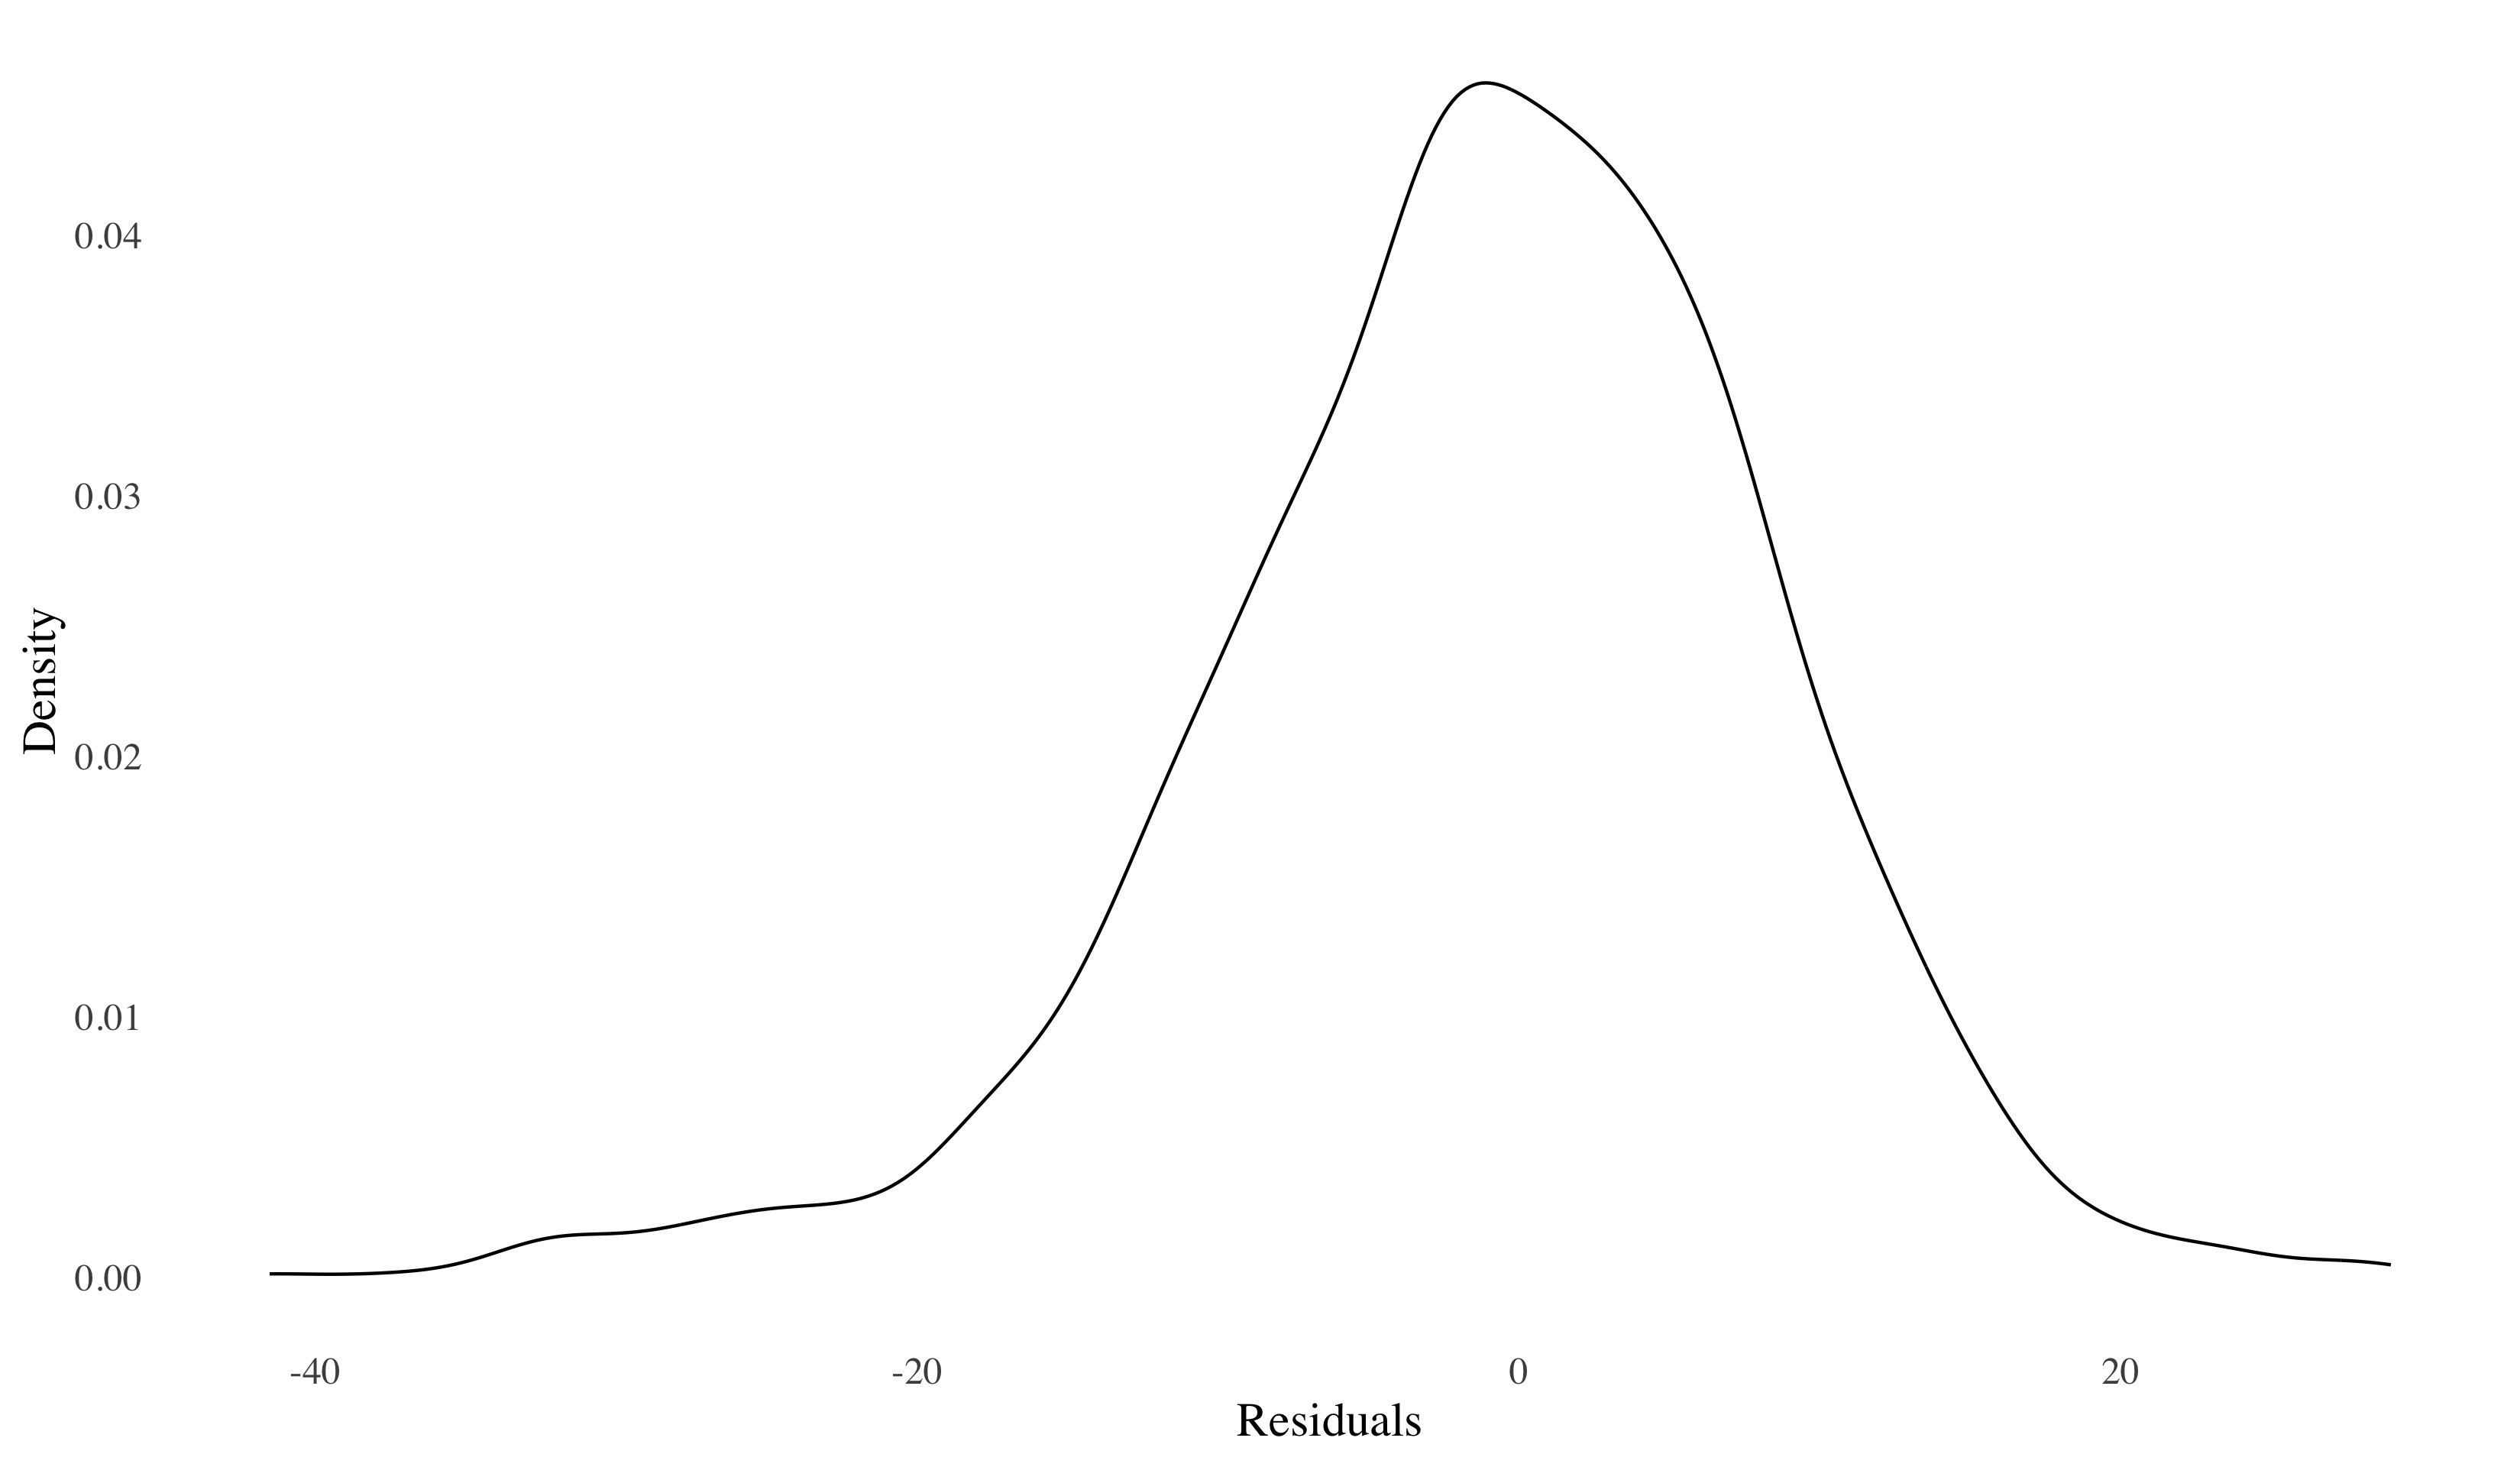
\includegraphics[scale = 0.14]{bayley_resids_plot}
\end{figure}

\end{document}